\documentclass[10pt,landscape,a4paper]{article}
\usepackage{multicol}
\usepackage{hyperref}
\usepackage[utf8]{inputenc}
\usepackage{minted}
\usepackage{venndiagram}
\usepackage{cancel}
\usepackage{wasysym}
\usepackage{amssymb}
\usepackage{stmaryrd}

\usepackage[top=5mm,bottom=1mm,left=5mm,right=5mm,includehead]{geometry}

%define header and footer
\usepackage{fancyhdr}
\pagestyle{fancy}

\fancyhead[RO]{\AUTHOR\hspace{4pt}|\hspace{4pt}\INSTITUTE}
\fancyhead[LO]{\TITLE}
\usepackage[style=iso]{datetime2}
\fancyfoot[RO]{\today}
\renewcommand\headrulewidth{0pt}
\renewcommand\footrulewidth{0pt}
\headsep = -2pt
\footskip = 0pt

% Graphics
\usepackage{graphicx}
\graphicspath{{graphics/}}

% Redefine section commands to use less space
\makeatletter
\renewcommand{\section}{\@startsection{section}{1}{0mm}%
    {-1ex plus -.5ex minus -.2ex}%
    {0.5ex plus .2ex}%x
    {\normalfont\large\bfseries}}
\renewcommand{\subsection}{\@startsection{subsection}{2}{0mm}%
    {-1explus -.5ex minus -.2ex}%
    {0.5ex plus .2ex}%
    {\normalfont\small\bfseries}}
\renewcommand{\subsubsection}{\@startsection{subsubsection}{3}{0mm}%
    {-1ex plus -.5ex minus -.2ex}%
    {1ex plus .2ex}%
    {\normalfont\footnotesize\bfseries}}
\renewcommand{\@venn@radius}{4mm}
\renewcommand{\@venn@overlap}{2mm}
\renewcommand{\@venn@vgap}{1mm}
\renewcommand{\@venn@hgap}{1mm}
\makeatother

% Don't print section numbers
\setcounter{secnumdepth}{0}

\setlength{\parindent}{0pt}
\setlength{\parskip}{0pt plus 0.5ex}

\newcommand{\sqljoin}[3]{
    \begin{multicols*}{2}
        \begin{venndiagram2sets}
            #1
        \end{venndiagram2sets}
        \vfill\columnbreak
        \hspace{-8em}
        \begin{tabular}{ll}
            x & y \\
            \hline
            #2
        \end{tabular}
    \end{multicols*}
    \mint{sql}{#3}
}

\newcommand{\sql}[1]{\mintinline{sql}{#1}}


\newcommand{\TITLE}{Datenbanksysteme 1}
\newcommand{\AUTHOR}{Florian Bruhin, Mona Panchaud}
\newcommand{\INSTITUTE}{Ostschweizer Fachhochschule}
\begin{document}

\footnotesize
\begin{multicols*}{3}

% multicol parameters
% These lengths are set only within the two main columns
%\setlength{\columnseprule}{0.25pt}
\setlength{\premulticols}{1pt}
\setlength{\postmulticols}{1pt}
\setlength{\multicolsep}{1pt}
\setlength{\columnsep}{2pt}

\section{Normalformen}
\begin{description}
    \item[1.NF] Wertebereiche der Tabelle sind atomar: strukturierte Werte (Mengen, Wiederholungsgruppen etc.) sind nicht zugelassen (z.B. nicht Vor-/Nachname in 1 Attribut), hat PK
    \item[2.NF] Every non-key attribute \textbf{must} depend on entire primary key
    \item[3.NF] Every non-key attribute should depend on key, the whole key, and nothing but the key. (keine transitiven Abhängigkeiten)
\end{description}

\section{Relationales Modell}

\texttt{Game (\underline{Id} INT PK, Name TEXT UNIQUE, Zu1Beziehung INT NOT NULL REFERENCES TblB, Zu0Beziehung INT REFERENCES TblC)}

\section{Abbildung}
\subsection{1:n/n:n Beziehungen}
1:n via Fremdschlüssel (oder Zwischentabelle mit Attributen), n:n via
Zwischentabelle.
\subsection{Vererbung}
\begin{description}
    \item[incomplete] only some instances of the parent class are specialized (have unique attributes)
    \item[complete] every instance of the parent class has one or more unique attributes that are not common to the parent class
    \item[overlapping] object could be a member of more than one specialized subclass
    \item[disjoint] object could be a member of only one specialized subclass
\end{description}
\vspace{3pt}
\begin{itemize}
\item Eine Tabelle für Sub-/Superklasse, mit enum: \\
    \sql{CREATE TYPE angtyp AS ENUM ('Chefin', 'Sysadmin')}
    \\
    Redundanzfrei. Auch für overlapping Vererbung geeignet.
    \\
    Viele Tabellen, Komplexe Zugriffe. Zusätzliches Typ Attribut.

\item Je eine Tabelle pro Subklasse\\
    Semantikverlust. Schlüssel-Eindeutigkeit ggf. über eigene Tabelle sicherstellen. Überlappende Vererbung kann nicht abgebildet werden.

\item Eine Superklasse-Tabelle mit allen Attributen (\verb!NULL!)\\
    Viele Null-Werte pro Tupel. Dritte oder höhere Normalform verletzt.
\end{itemize}

\section{SQL DDL (Data Definition Language)}

\begin{minted}{sql}
CREATE DATABASE foo WITH OWNER = 'bar';
CREATE TABLE Game (
  ArticleID INTEGER PRIMARY KEY,
  Name VARCHAR(300) NOT NULL,
  Date DATE DEFAULT CURRENT_DATE,
  FK_FOO INTEGER NOT NULL REFERENCES FooTable (id)
  ...  -- ggf. constraints, ohne "ADD CONSTRAINT"
);
\end{minted}

\begin{minted}{sql}
ALTER TABLE Game
  ADD Kuerzel TYPE CHAR;
  ALTER COLUMN Date TYPE STRING;
\end{minted}

\begin{minted}{sql}
ALTER TABLE AbtLeitung
  ADD CONSTRAINT fk_AbtLAbt
    FOREIGN KEY (AbtNr) REFERENCES Abteilung (AbtNr)
    -- AbtLeitung wird gelöscht wenn Abteilung gelöscht wird
    ON DELETE CASCADE;

... CHECK (Salaer BETWEEN 1000 and 20000);

CREATE INDEX name ON tbl (col);
  WHERE state = 'N'; -- partiell

DROP CONSTRAINT fk_AbtLAbt;
\end{minted}

% TODO keep this or drop?
Index Gründe
\begin{itemize}
    \item Index Only Scan kann verwendet werden
    \item Where Condition kann aufgrund B-Tree schneller ausgewertet werden
    \item Sortieren geht schneller, da Werte in B-Tree bereits sortiert
\end{itemize}

ON DELETE:

\begin{itemize}
  \item \sql{CASCADE}: Tupel mit Fremdschlüssel werden gelöscht
  \item \sql{NO ACTION / RESTRICT}: Fehler/Rollback
  \item \sql{SET NULL}
  \item \sql{SET DEFAULT}
\end{itemize}

\section{SQL DML (Manipulation)}
\begin{minted}{sql}
INSERT INTO abteilung VALUES (1, 'Verkauf');
UPDATE Ang set salaer = 30000 WHERE persnr = 1100;
DELETE FROM Mitarbeiter WHERE Abteilung_ID = 1;
\end{minted}

\section{SQL DQL (Query)}

\subsection{Select}
\begin{minted}{sql}
SELECT DISTINCT Wohnort, Name FROM angestellter
WHERE AbtNr=3 AND Name LIKE 'Mo%'
ORDER BY Wohnort ASC, Name DESC;
\end{minted}

\subsubsection{korrelierte Unterabfrage}

\begin{minted}[escapeinside=||]{sql}
SELECT * from Products p WHERE Quantity <
 (SELECT AVG(Quantity) FROM Items s WHERE |\colorbox{yellow}{p.ID}| = s.ID);
\end{minted}

\begin{description}
\item[Projektion]{$\pi_{\mathrm{foo, bar}}(A)$ \\
    \sql{SELECT foo, bar FROM A;}}
\item[Selektion]{$\sigma_{\mathrm{ID < 10}}(A)$ \\
    \sql{SELECT * FROM A WHERE ID < 10;}}
\item[Umbenennung]{$\rho_{\mathrm{foo} \leftarrow \mathrm{bar}}$ \\
  \sql{SELECT foo AS bar FROM ...;}}
\item[Vereinigung]{$A \cup B$ \\
    \sql{SELECT * FROM A UNION [ALL] SELECT * FROM b;}}
\item[Durchschnitt]{$A \cap B$ \\
    \sql{SELECT * FROM A INTERSECT SELECT * FROM b;}}
\end{description}

\subsection{Join ($\bowtie$)}

\texttt{a.x}: 1, 2 \hspace{2em} \texttt{b.y}: 2, 3

\subsubsection{Inner Join}
\sqljoin{\fillACapB}{2 & 2}{SELECT * FROM a INNER JOIN b ON a.x = b.y;}

\subsubsection{Left Join}
\sqljoin{\fillA}{1 & \texttt{NULL} \\ 2 & 2}{SELECT * FROM a LEFT JOIN b ON a.x = b.x;}
right: dito.
Mit \sql{WHERE b.x IS NOT NULL}: ohne $A \cap B$

\subsubsection{Outer join}
\sqljoin{\fillA \fillB}{1 & \texttt{NULL} \\ 2 & 2 \\ \texttt{NULL} & 3}{SELECT * FROM a FULL OUTER JOIN b ON a.x = b.x;}

\subsubsection{Andere}
\begin{description}
\item[natural]{Joinen nach gleichnamigen Attributen, Spalten nur 1x im Resultat}
\item[theta]{RelAlg: join-operator $\Theta \in \{<, \leq, =, \geq, >\}$}
\item[equi]{Join mit \verb|colA = colB|}
\end{description}

\subsection{Group By}
\begin{minted}{sql}
SELECT AVG(Lohn) FROM Ang
GROUP BY Abtnr HAVING AVG(Lohn) > 7000;
\end{minted}

Aggregate functions: \sql{COUNT, FIRST, LAST, MAX, MIN, SUM, AVG} \\
\sql{NULL} wird übersprungen/nicht gezählt

\subsection{Window functions}
\begin{minted}{sql}
SELECT abtnr, MAX(salaer) OVER (PARTITION BY abtnr) FROM Ang;
\end{minted}

Tupel werden beibehalten, wir machen nur eine neue Spalte mit dem maximalen
Salär (Wert ggf. wiederholt).

\subsubsection{rank / lead / lag}
\begin{minted}{sql}
SELECT name, preis, rank() OVER(ORDER BY preis DESC)
FROM game LIMIT 5;  -- 5 teuerste Games
SELECT *, (LEAD(ankunftsZeit) OVER () - abfahrtsZeit)::time as x
FROM fahrplan; -- Fahrtdauer
\end{minted}

\begin{description}
  \item[lag(val, offset=1, default=NULL)]{Wert von \emph{offset} Reihen vorher
      (\textbf{lead}: Nachher)}
\end{description}

\subsection{Views}
\sql{CREATE VIEW name AS SELECT ...;}

Updatable: Kein \sql{FROM}-Eintrag; kein with, distinct, group by, having,
limit, offset, union, except, intersect; selbige Spalte nicht mehrmals

\subsection{CTE}
\begin{minted}{sql}
WITH tmp AS (SELECT ...) SELECT * FROM tmp;
\end{minted}

Rekursiv:

\begin{minted}{sql}
WITH RECURSIVE cte (spalten) AS
   (Ursprungsselect UNION ALL Rekursionsselect)
SELECT spalten FROM cte WHERE ...;
\end{minted}

Beispiel:

\begin{minted}{sql}
WITH RECURSIVE unter ( persnr, name, chef ) AS
   (SELECT A.persnr, A.name, A.chef FROM angestellter A
    WHERE A.chef = 1010    UNION ALL
    SELECT A.persnr, A.name, A.chef FROM angestellter A
    INNER JOIN unter B on B.persnr = A.chef
) SELECT * FROM unter ORDER BY chef, persnr;
\end{minted}

\subsection{Varia}

\begin{description}
\item[Scalar fns]{\sql{[U/L]CASE}, \sql{MID(n, s, len)}, \sql{LEN}, \sql{ROUND}, $\ldots$}
\item[EXISTS]{\sql{SELECT * FROM a WHERE EXISTS (SELECT ...)};}
\item[ANY/ALL]{\sql{SELECT * FROM a WHERE a.x < ANY (SELECT ...)};}
\item[IN]{\sql{SELECT * FROM a WHERE a.x IN (1, 2);}}
\item[CAST]{\sql{SELECT CAST(CASE WHEN tot IS NULL THEN 1 ELSE 0 END} \\ \sql{AS
      BOOLEAN);} - alternativ: \sql{(tot IS NULL) AS foo;}}
\item[COALESCE]{\sql{COALESCE(n1, n2, "def");}, erster non-NULL Wert}
\item[3-Werte-Logik]{true/false/unknown. Skalarer Ausdruck/Vergleich mit NULL: NULL.}
\item[Alter]{\sql{SELECT ((current_date - gebdat) / 365) AS Alter}}
\end{description}

\section{SQL DCL (Control)}
\begin{minted}{sql}
CREATE ROLE angguest
    [WITH LOGIN PASSWORD 'hunter2'] [IN ROLE clients];
GRANT CREATE, INSERT, SELECT, UPDATE ON myTable TO myuser;
GRANT ALL ON [TABLE | SCHEMA | DATABASE] objectName
    TO angguest WITH GRANT OPTION;
GRANT myGroup TO angguest;
ALTER GROUP clients ADD USER user;
REVOKE UPDATE ON myTable FROM angguest;
\end{minted}

\section{Transactions}
\begin{minted}[escapeinside=||]{sql}
BEGIN TRANSACTION;
    SET TRANSACTION ISOLATION LEVEL SERIALIZABLE;
    INSERT INTO Ang (...) VALUES (...);
    SAVEPOINT ang_ok;
    UPDATE Ang SET ...;
    ROLLBACK TO SAVEPOINT ang_ok;
COMMIT TRANSACTION;
\end{minted}


\subsection{Serialisierbarkeit}
$r_{1}(x)$: T1 liest x / $w_{1}(x)$: T1 schreibt x / $c_{1}$: T1 commit

Konfliktpotential: 2 Transaktionen, write involviert, dasselbe Obj

\newcommand{\ta}[2]{{\color{blue}#1_{1}#2}}
\newcommand{\tb}[2]{{\color{red}#1_{2}#2}}
\newcommand{\tc}[2]{{\color{green}#1_{3}#2}}

\subsubsection{Schedule}
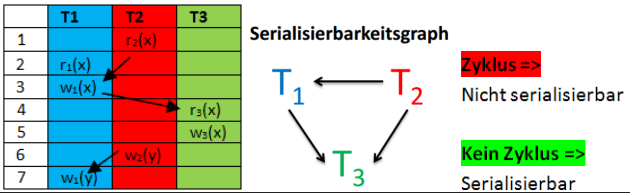
\includegraphics[width=20em]{serial.png}

\subsection{Isolationsverfahren}

\begin{description}
\item[2-Phase-Locking (2PL)]{Growing/Shrinking Phase: Vor Zugriff muss Objekt in Transaktion gesperrt werden. Sobald ein Lock freigegeben, dürfen keine weiteren mehr bezogen werden. Strict 2PL: Unlocks werden ganz am Ende von Transaktion freigegeben.}
\item[Opfersuche]{Zyklus unterbrechen $\rightarrow$ (ggf. cascading) rollback}
\item[Snapshot Isolation (SI)] von ganzer Tabelle wird 'Schattenkopie' angelegt
\item[MVCC] Nur von bearbeiteter Zeile wird 'Schattenkopie' angelegt.
Beim Schreiben werden Tupels mit x-Locks versehen. Beim Lesen werden keine Locks gesetzt/überprüft. Bei Änderungen im Commit prüfen, dass Objekte noch
unverändert wie zum Snapshot-Zeitpunkt sind, sonst Rollback.
\item[Deadlock-Voraussetzungen] mutex, geschachtelte locks, zyklisches Warten, locks ohne timeout
\item[Locks] \emph{slock} nur lesend (shared mit reader) \emph{xlock} exklusiv
\item[Optimistisches Locking] Prognose: Wenig writes. Kein slock, aber Zeitstempel prüfen.
\item[Pessimistisches Locking] Prognose: Viel writes. slock und xlock.
\end{description}

\checked: möglich; -: unmöglich

\begin{tabular}{p{70pt}p{40pt}p{30pt}p{40pt}p{40pt}}
    . & Garantiert Serialisierbarkeit & Deadlocks & Cascading Rollbacks & Konflikt-Rollbacks \\
    % . & . & . & . & . \\
    \hline
    2PL & \checked & \checked & \checked & - \\
    Strict 2PL & \checked & \checked & - & - \\
    Preclaiming 2PL & \checked & - & - & - \\
    Snapshot Isolation & - & \checked & - & \checked \\
    SSI & \checked & \checked & - & \checked \\
\end{tabular}

\subsection{Isolation levels}

\begin{description}
    \item[Dirty Read] Daten von nicht commiteter Transaktion werden gelesen. Andere Transaktion macht zB Rollback, es werden falsche Berechnungen gemacht.
    \item[Fuzzy Read (Non-Repeatable read)] Gleiche Daten werden mehrmals gelesen, aber sind anders, da Werte durch nebenläufige Transaktionen verändert wurden.
    \item[Phantom Read] Select in Tabelle => neue oder gelöschte Rows werden entdeckt.
\end{description}

\checked: möglich; -: unmöglich

\begin{tabular}{lllll}
  Isolation & Dirty & Fuzzy & Phantom & Write Skew \\
  \hline
  Read uncommited & \checked & \checked & \checked & \checked \\
  \textbf{Read committed} & - & \checked & \checked & \checked \\
  Repeatable read & - & - & \checked & \checked \\
  Serializable & - & - & - & \checked
\end{tabular}

\subsection{Fehlerbehandlung}
WAL (write ahead log): Zuerst Log schreiben, dann commit.

Loganalyse $\rightarrow$ Fertige Transaktionen \emph{redo}, angebrochene
Transaktionen \emph{undo}

Loginhalt: [LSN (sequence number), TransaktionsID, PageID, Redo (SQL),
Undo (SQL), PrevLSN]

\section{B-Tree (Balanced-Tree)}

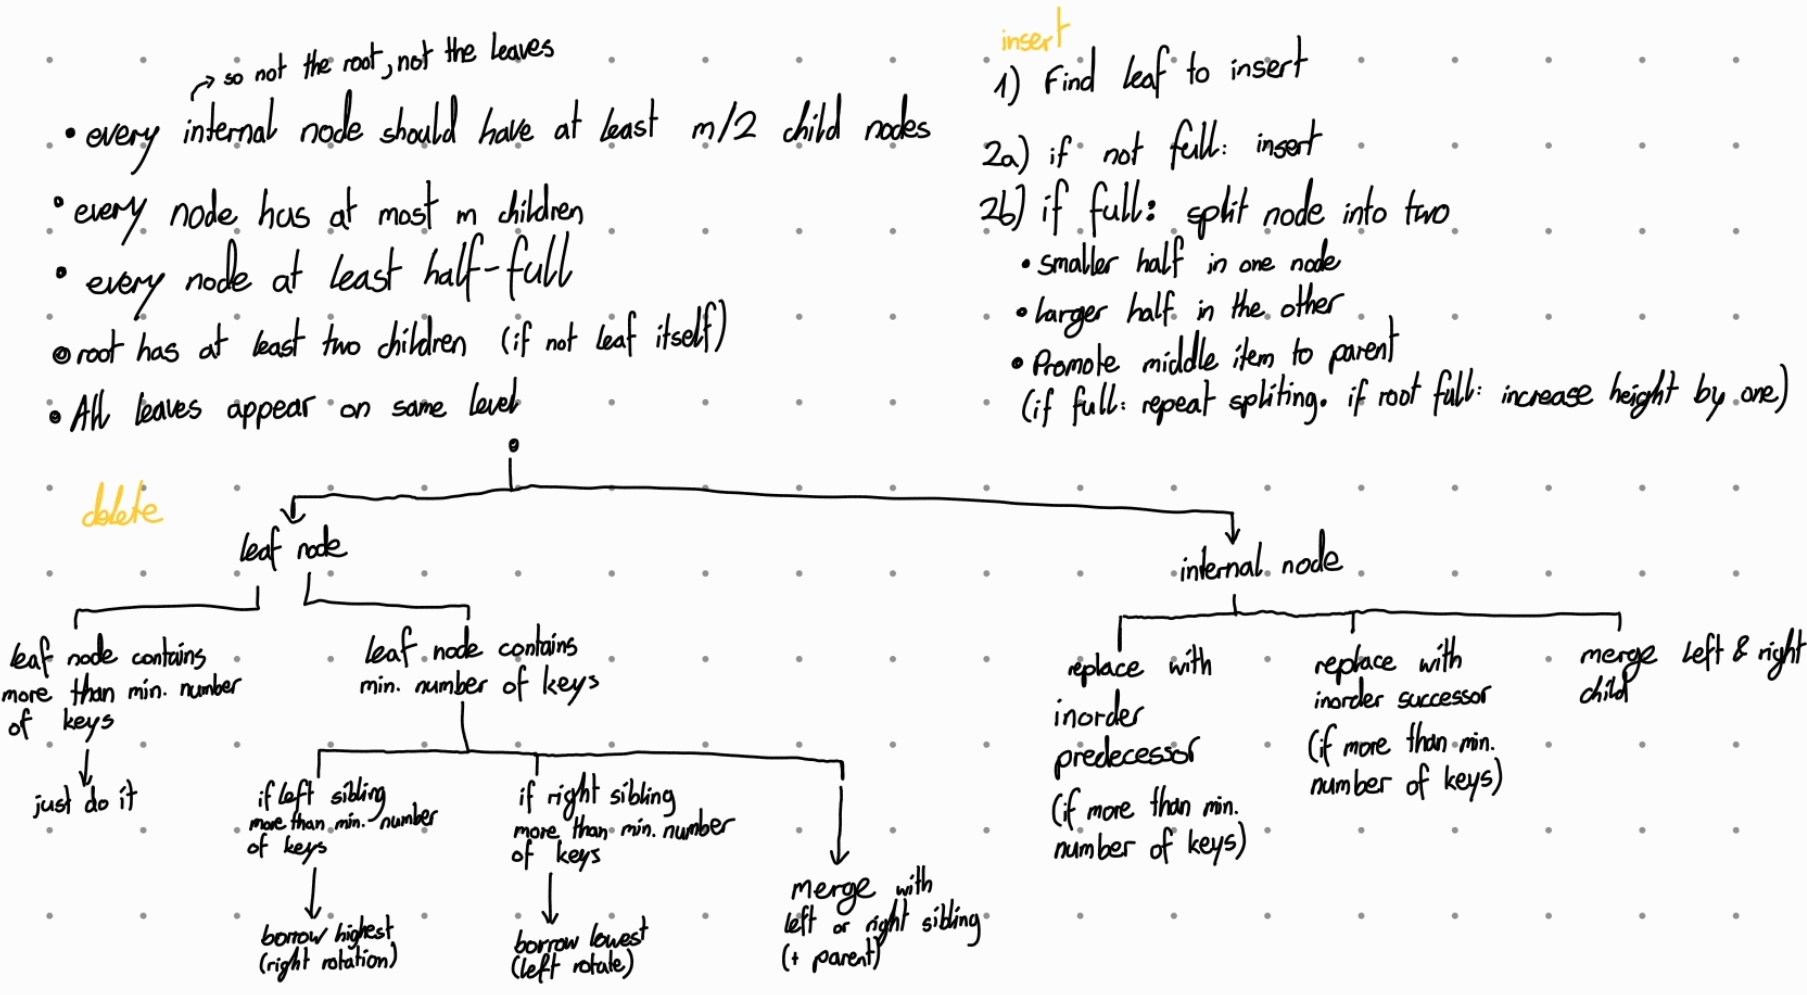
\includegraphics[width=\columnwidth]{b_tree.jpg}

\section{UML}

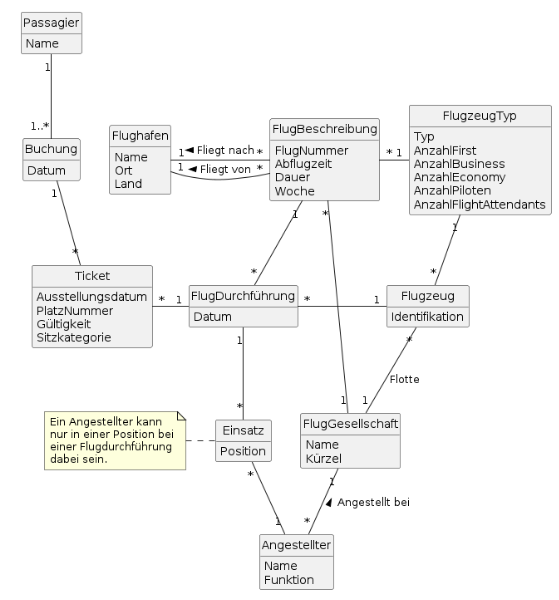
\includegraphics[height=\columnwidth-2em,angle=90]{uml2.png}

Aggregation: $\lozenge$ Komposition: $\blacklozenge $

Vererbung mit subclass {\huge$\rightarrowtriangle$} superclass.

\section{Begriffe}

\begin{description}
\item[Vorteile]{Skalierbar, Permissions, Integrität, Live-Abfragen, Kapslung}
\item[Funktionen]{Transaktionen, Mehrbenutzer, Backups, $\ldots$}
\item[3-Ebenen]{\emph{externe Ebene} (Anwendungen-Sicht), \emph{logische (konzeptionale) Ebene}
    (DB/konzeptionelles Schema, letzteres ist Modell der Realität), \emph{interne
    Ebene}. Durch Trennung: Datenunabhängigkeit}
\item[Datenbasis]{Daten auf HDD - Anwendungsdaten und Data Dictionary (Metadaten)}
\item[Entitätstyp]{Klasse}
\item[Schlüsselkandidaten]{Minimale Attributskombinationen, die eine Entität
    gerade noch eindeutig identifizieren}
\item[ACID]{Atomicity (Transaktion wird entweder vollständig oder gar nicht ausgeführt), Consistency, Isolation, Durability}
\item[Indexe]{ISAM (Aufsteigend via Indexspalte, überlaufseiten möglich), Hash, BRIN, GiST, GIN, Btree, Bitmap. Kann funktional/zusammengesetzt/partiell/clustered sein.}
\item[Mutationsanomalien]{Bei Redundanz. INSERT-, UPDATE-, DELETE-Anomalie}
\item[Surrogatschlüssel]{Künstlicher Schlüssel, z.B. für Performance bei
    zusammengesetztem Schlüssel}.
\end{description}


\end{multicols*}
\end{document}
